\chapter{Survey two results and analysis}
\label{chap:Survey two results and analysis}
\lhead{\emph{Survey two results and analysis}}

\section{Survey two results}

Survey two is the Autism and Assistive Technology Survey, this survey involved 11 participants who all had relationships with individuals who were Autistic, worked with Autistic individuals, had a family member who was Autistic, had Autism themselves or had a close contact who was Autistic. 

\begin{figure}[b]
\centering
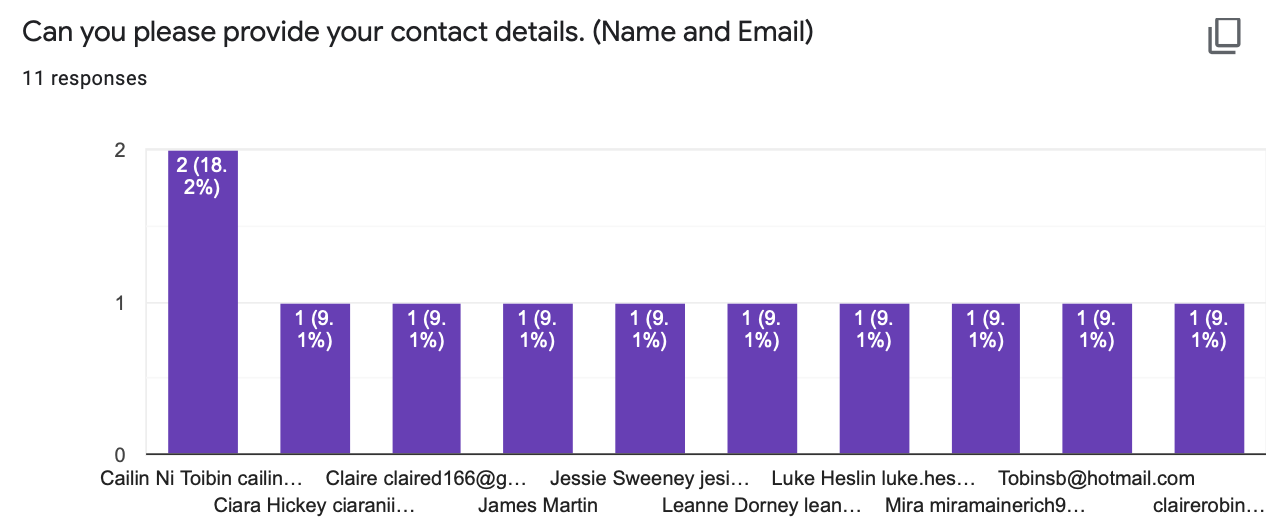
\includegraphics[width=1.0\textwidth]{IDD_LauraMartin_R00124705/Figures/respondentsSurvey2.png}
\caption{Details of participants}
{For question one, 11 respondents gave their name and email addresses.}
\end{figure}

\begin{figure}[b]
\centering
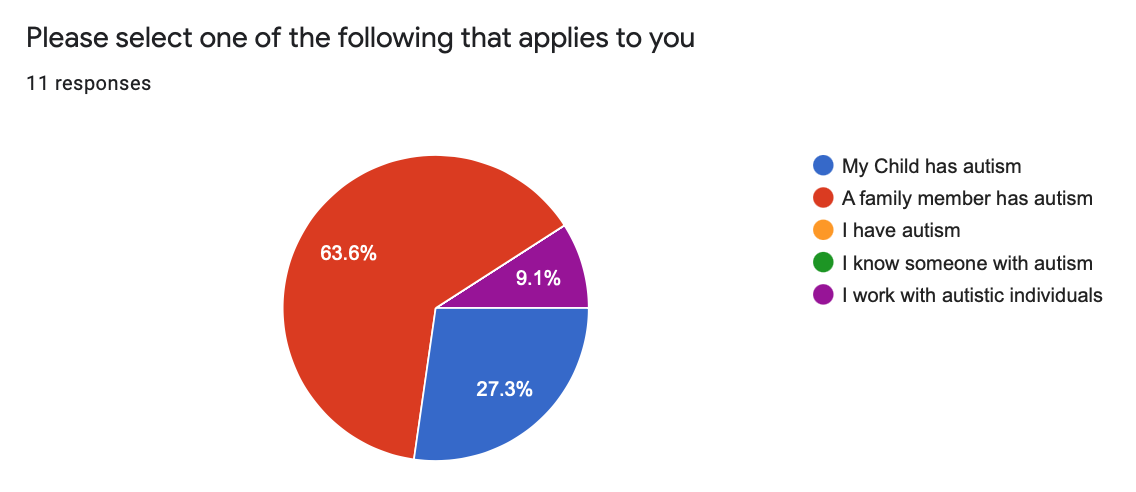
\includegraphics[width=1.0\textwidth]{IDD_LauraMartin_R00124705/Figures/survey1.png}
\caption{Relationship between respondent and person with Autism}
{For question two, 11 respondents answered their relationship to a person with Autism. The highest answer was the respondents have a family member with Autism, followed by their Child is Autistic and finally the respondents work with individuals who are Autistic}
\end{figure}


\begin{figure}[b]
\centering
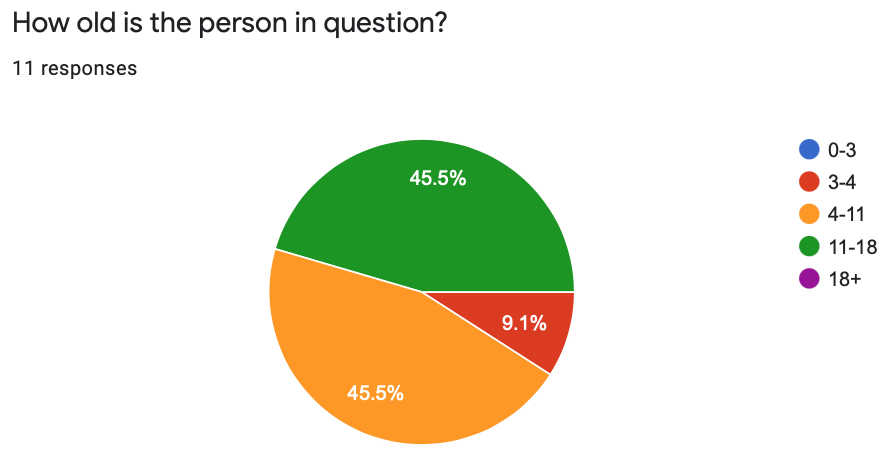
\includegraphics[width=1.0\textwidth]{IDD_LauraMartin_R00124705/Figures/survey2.png}
\caption{Pie chart representing the age of the individual with Autism.}
{For question three, 11 respondents answered a multiple choice question about their relationship to a person with Autism. The highest ages were those of school going ages. Ages between 11-18 was the most common, 4-11 was second and the least common was age 3-4 years old.}
\end{figure}


\begin{figure}[b]
\centering
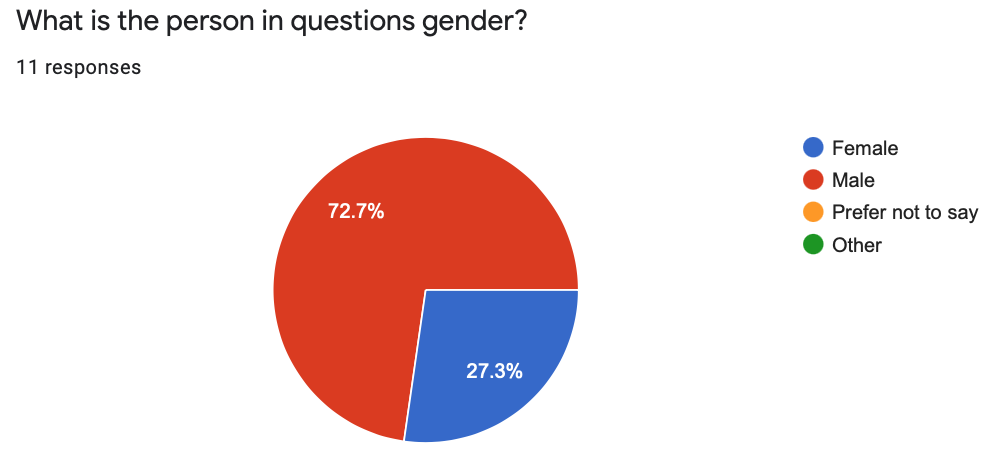
\includegraphics[width=1.0\textwidth]{IDD_LauraMartin_R00124705/Figures/survey3.png}
\caption{Pie chart representing the person in questions gender}
{For question four, 11 respondents answered a multiple choice question about the age of the person with Autism. The highest gender was Male at 72.7 percent and followed by female at 27.3 percent.}
\end{figure}

\begin{figure}[b]
\centering
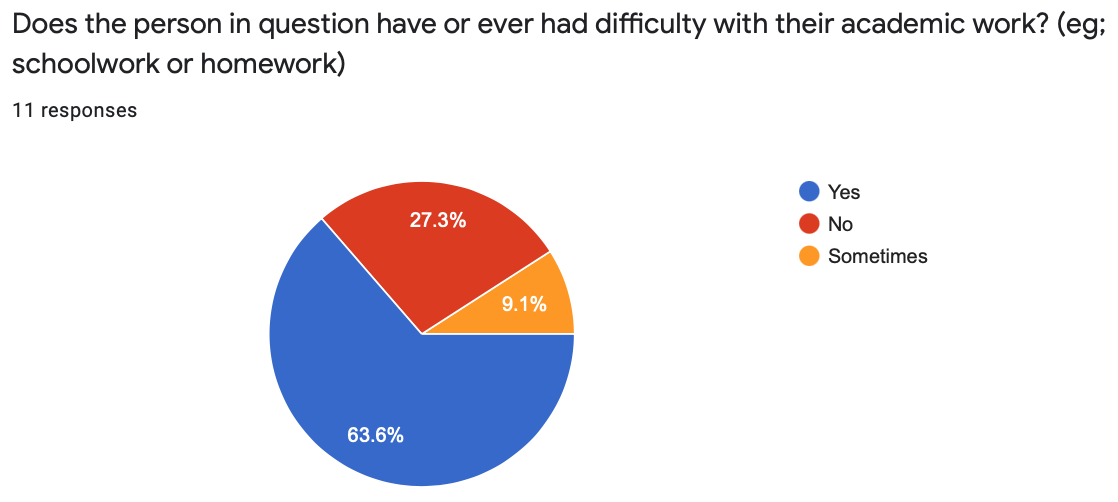
\includegraphics[width=1.0\textwidth]{IDD_LauraMartin_R00124705/Figures/survey4.png}
\caption{Pie chart representing the person in questions academic ability}
{For question five, 11 respondents answered a multiple choice question about the Autistic person in question and their ability in relation to their academic work.}
\end{figure}

\begin{figure}[b]
\centering
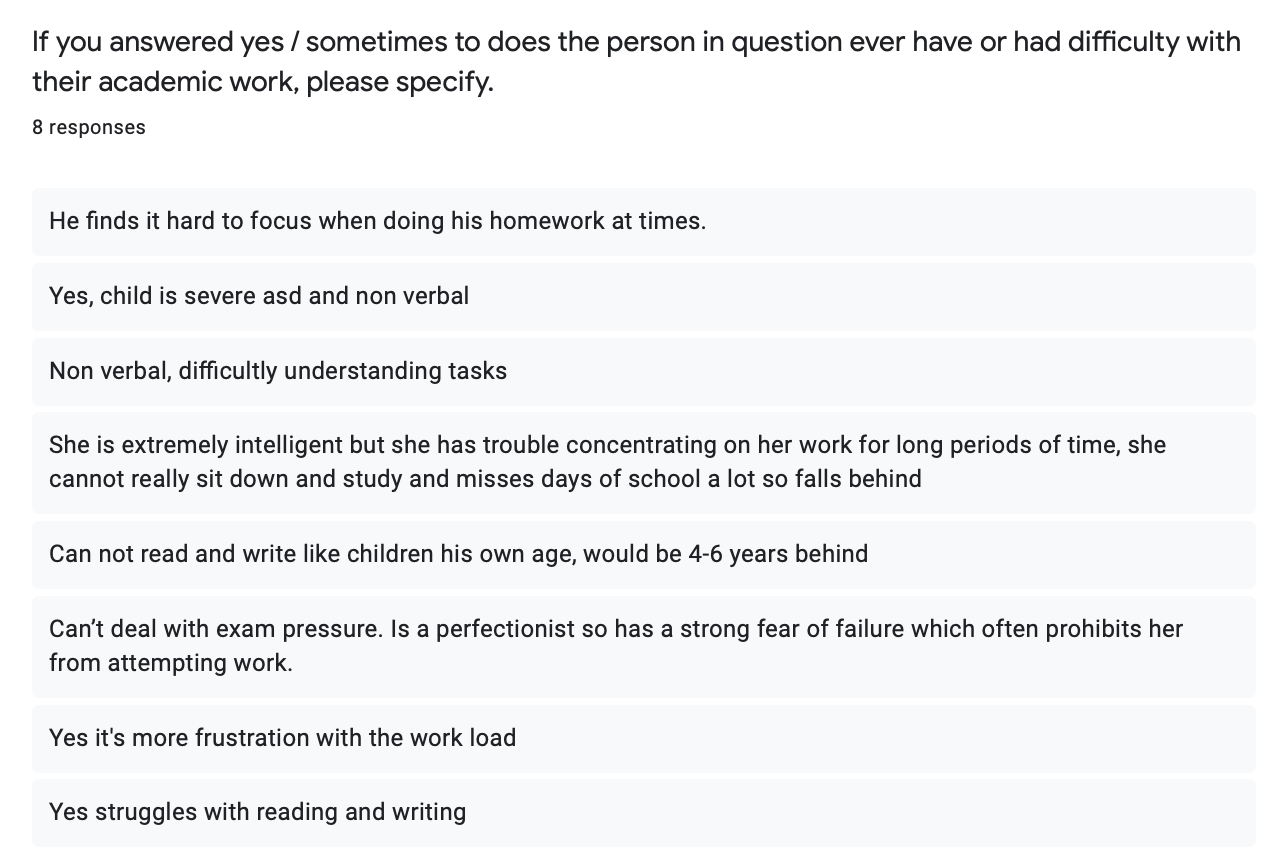
\includegraphics[width=1.0\textwidth]{IDD_LauraMartin_R00124705/Figures/academicdifficulty.png}
\caption{Academic difficulty answer box}
{For question six, 8 respondents were able to specify why the person with Autism does or sometimes struggles with their academic work.}
\end{figure}

\begin{figure}[b]
\centering
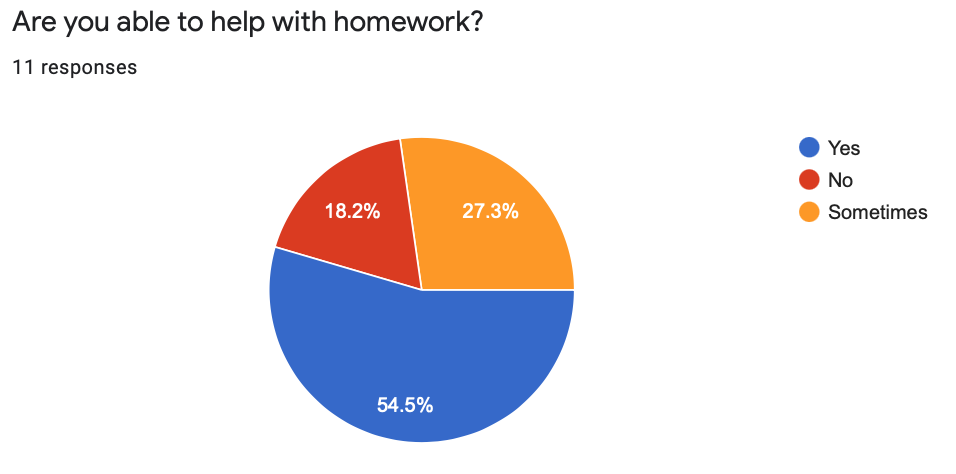
\includegraphics[width=1.0\textwidth]{IDD_LauraMartin_R00124705/Figures/survey5.png}
\caption{Does the respondent help with homework pie chart}
{For question seven, 11 respondents were given multiple choice questions about their ability to help the person in question with their homework.}
\end{figure}

\begin{figure}[b]
\centering
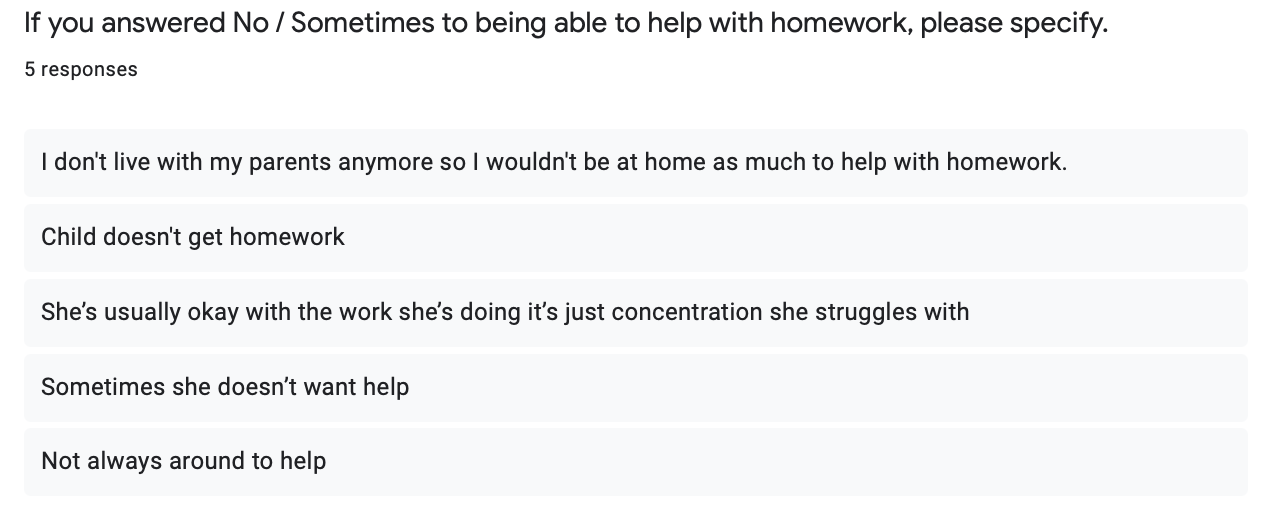
\includegraphics[width=1.0\textwidth]{IDD_LauraMartin_R00124705/Figures/homeworkhelp.png}
\caption{Helping with homework answer box}
{For question eight, 5 respondents gave their answer as to why they can not or only sometimes help the person with Autism and their homework. }
\end{figure}

\begin{figure}[b]
\centering
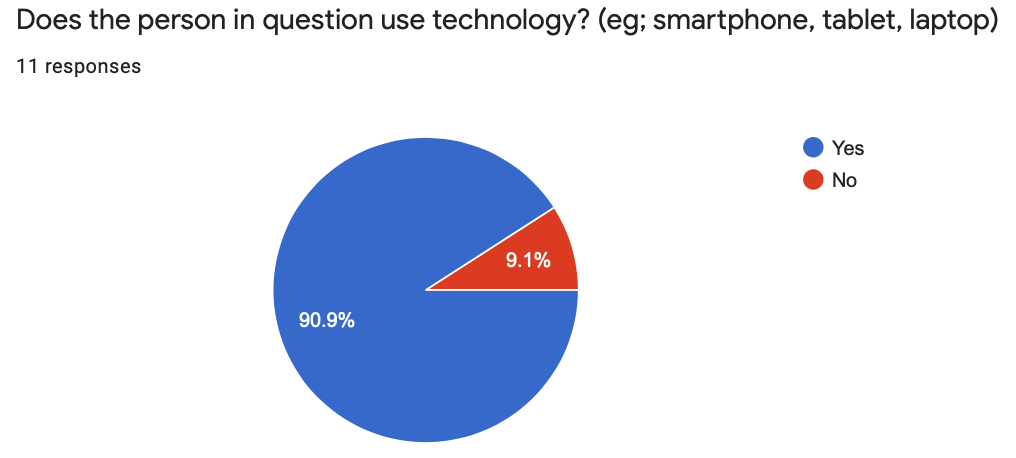
\includegraphics[width=1.0\textwidth]{IDD_LauraMartin_R00124705/Figures/survey6.png}
\caption{Does the person use technology}
{For question nine, 11 respondents answered does the person in question use technology.}
\end{figure}

\begin{figure}[b]
\centering
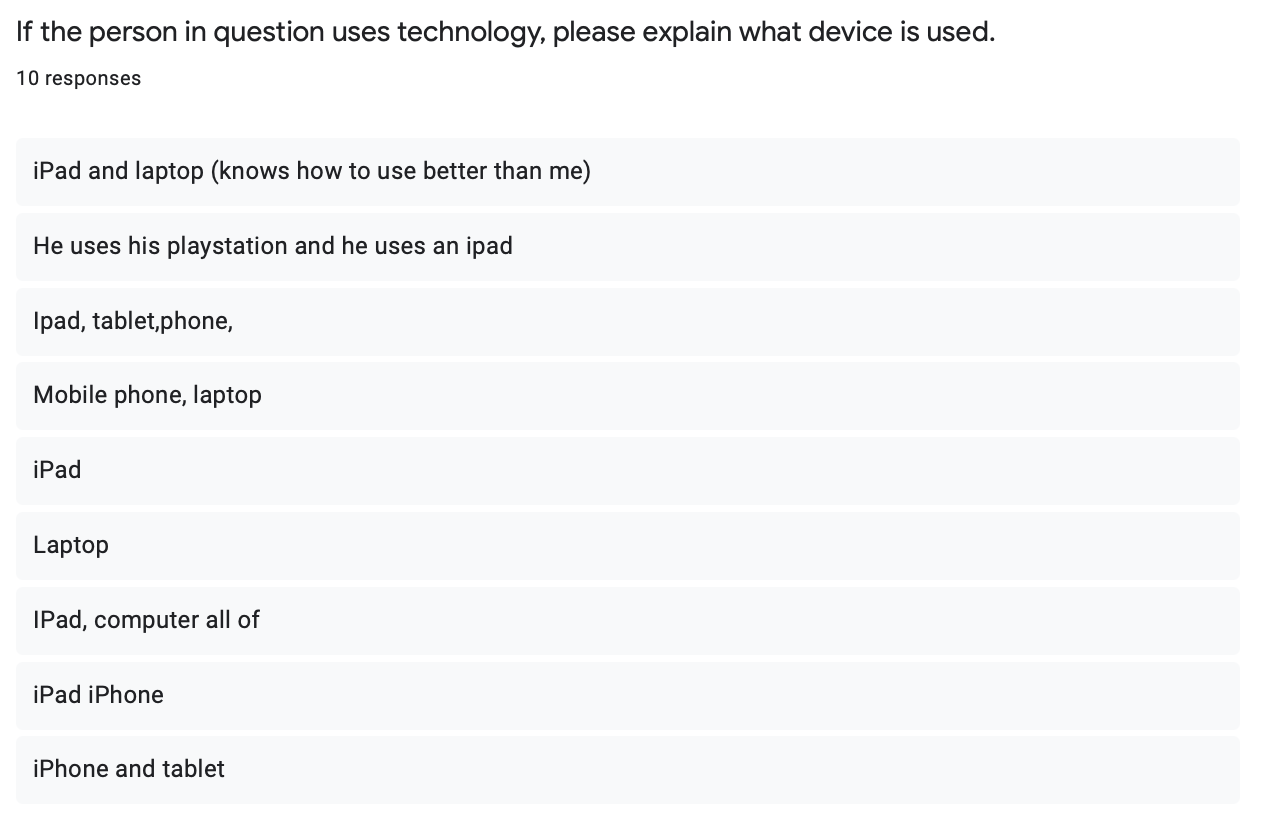
\includegraphics[width=1.0\textwidth]{IDD_LauraMartin_R00124705/Figures/technologyused.png}
\caption{What devices are used answer box}
{For question ten, 10 respondents answered what devices the person in question uses.}
\end{figure}

\begin{figure}[b]
\centering
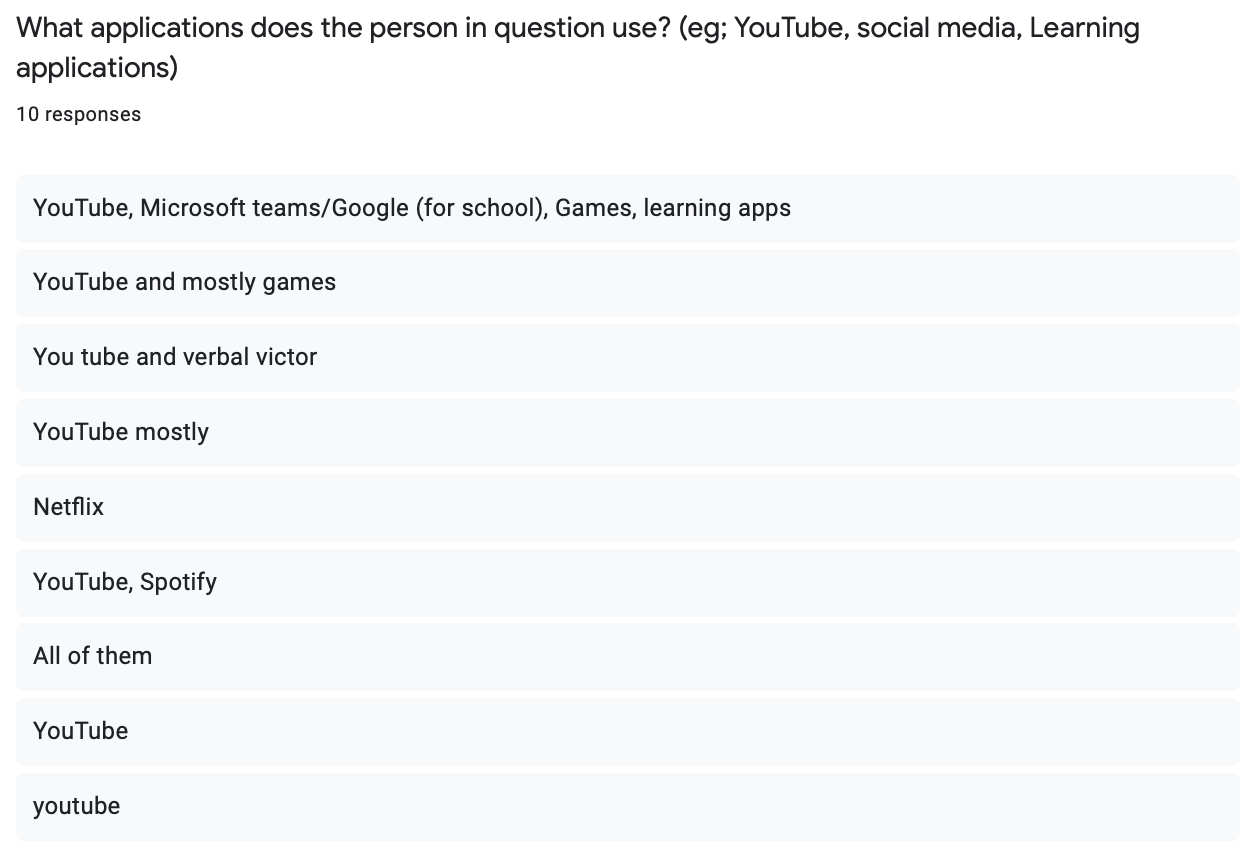
\includegraphics[width=1.0\textwidth]{IDD_LauraMartin_R00124705/Figures/applicationsused.png}
\caption{What applications are used answer box}
{For question eleven, 10 respondents answered what applications the person in question uses. }
\end{figure}

\begin{figure}[b]
\centering
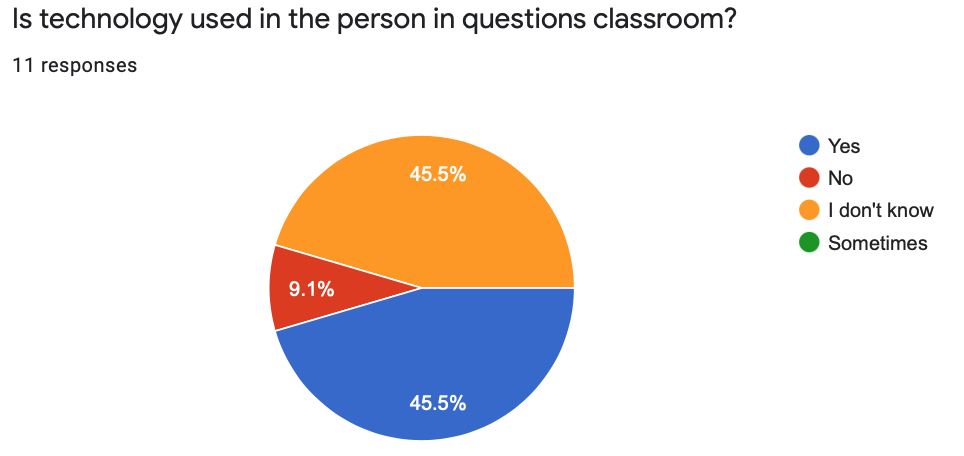
\includegraphics[width=1.0\textwidth]{IDD_LauraMartin_R00124705/Figures/survey7.png}
\caption{What devices are used pie chart}
{For question twelve, 11 respondents answered is technology used in the classroom of the individual with Autism. }
\end{figure}

\begin{figure}[b]
\centering
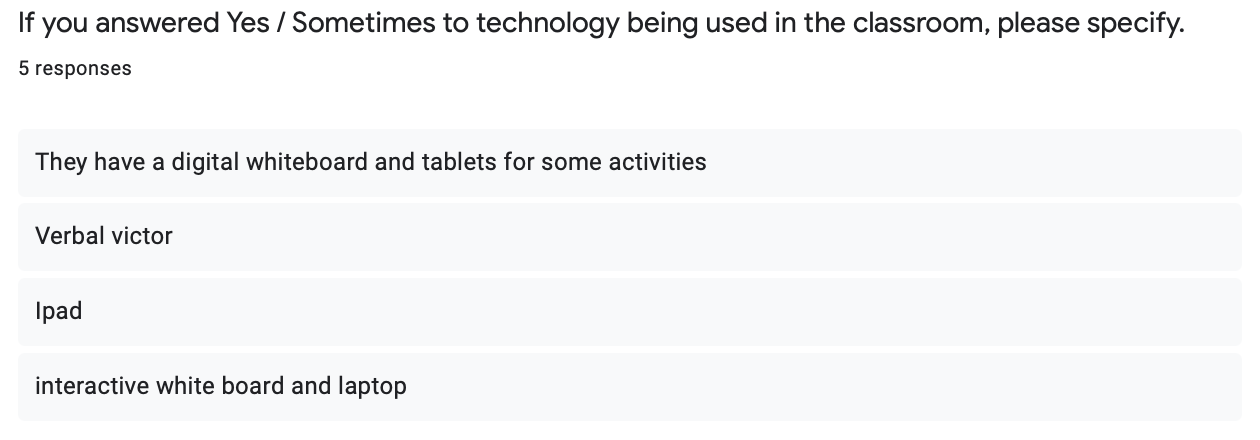
\includegraphics[width=1.0\textwidth]{IDD_LauraMartin_R00124705/Figures/classtechnology.png}
\caption{what technology is used answer box}
{For question thirteen, 5 respondents answered what technology devices are used in the classroom of the individual with Autism. }
\end{figure}

\begin{figure}[b]
\centering
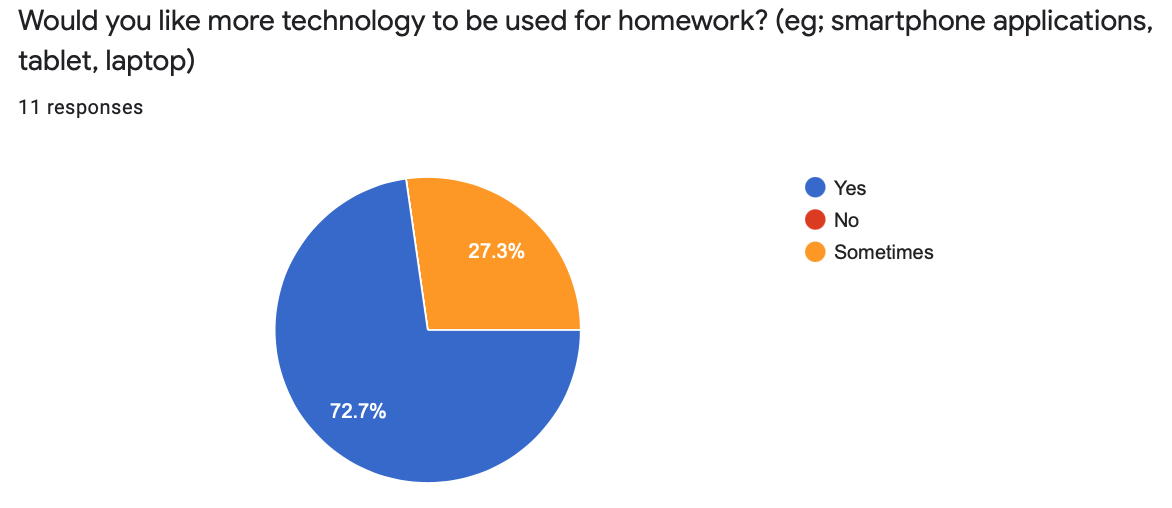
\includegraphics[width=1.0\textwidth]{IDD_LauraMartin_R00124705/Figures/survey8.png}
\caption{Technology devices pie chart}
{For question fourteen, 5 respondents answered what technology devices are used in the classroom of the individual with Autism. }
\end{figure}

\begin{figure}[b]
\centering
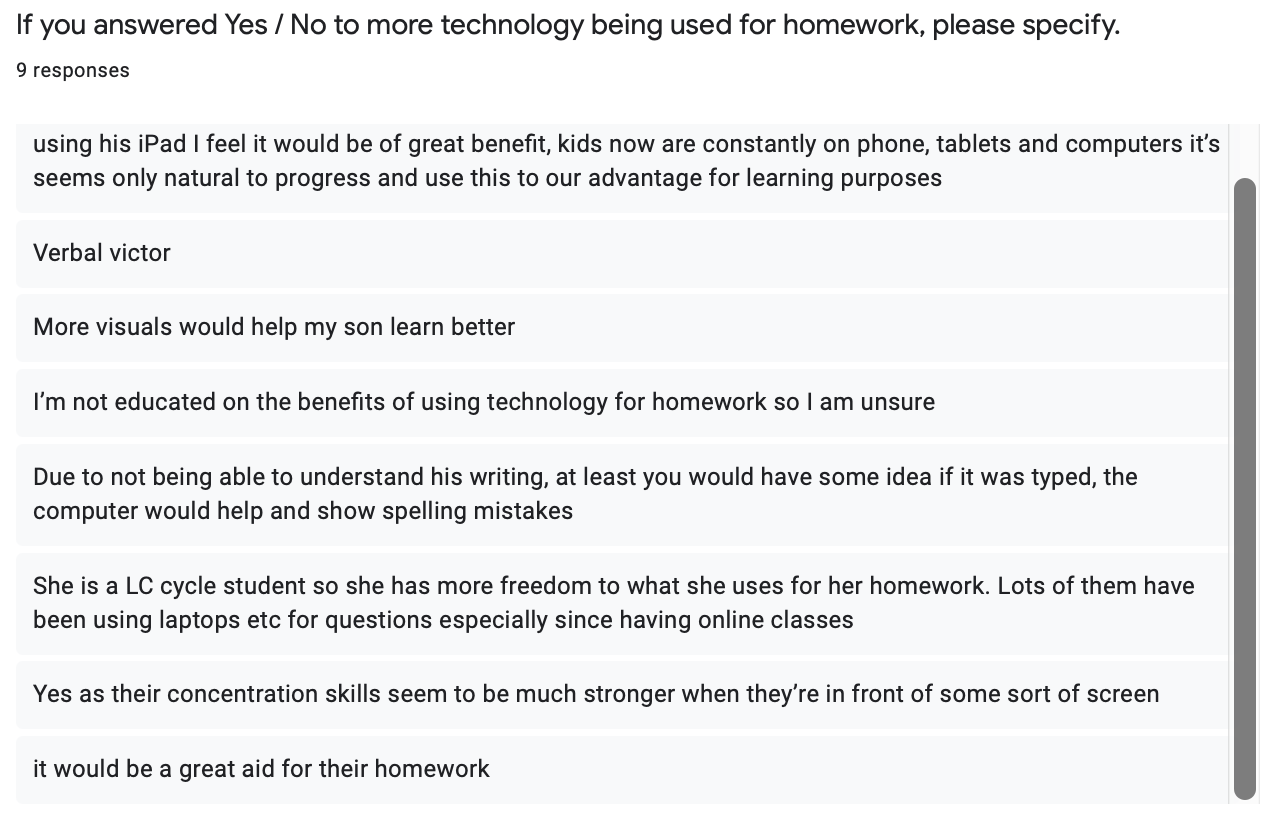
\includegraphics[width=1.0\textwidth]{IDD_LauraMartin_R00124705/Figures/moretechnologyused.png}
\caption{More technology answer box}
{For question fifteen, 9 respondents answered why more or less technology devices should be used for the person in question education. }
\end{figure}

\begin{figure}[b]
\centering
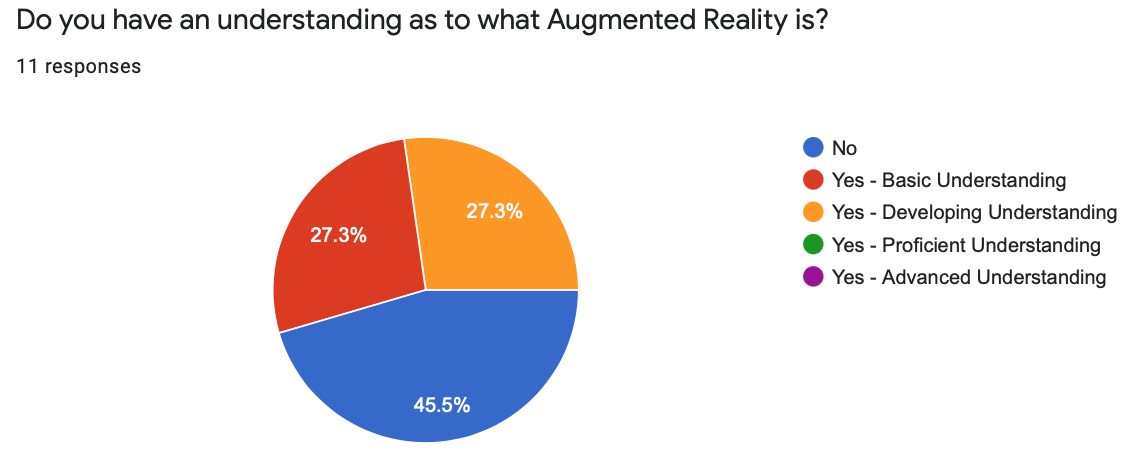
\includegraphics[width=1.0\textwidth]{IDD_LauraMartin_R00124705/Figures/survey9.png}
\caption{AR understanding Pie chart}
{For question sixteen, 11 respondents were given a multiple question about their understanding of AR.}
\end{figure}

\begin{figure}[b]
\centering
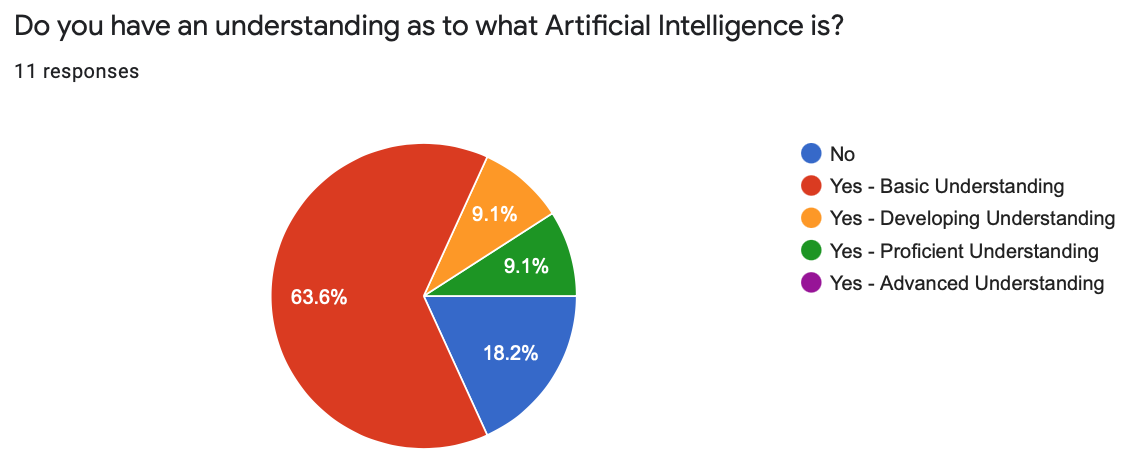
\includegraphics[width=1.0\textwidth]{IDD_LauraMartin_R00124705/Figures/survey10.png}
\caption{AI understanding Pie chart}
{For question seventeen, 11 respondents were given a multiple question about their understanding of AI.}
\end{figure}

\begin{figure}[b]
\centering
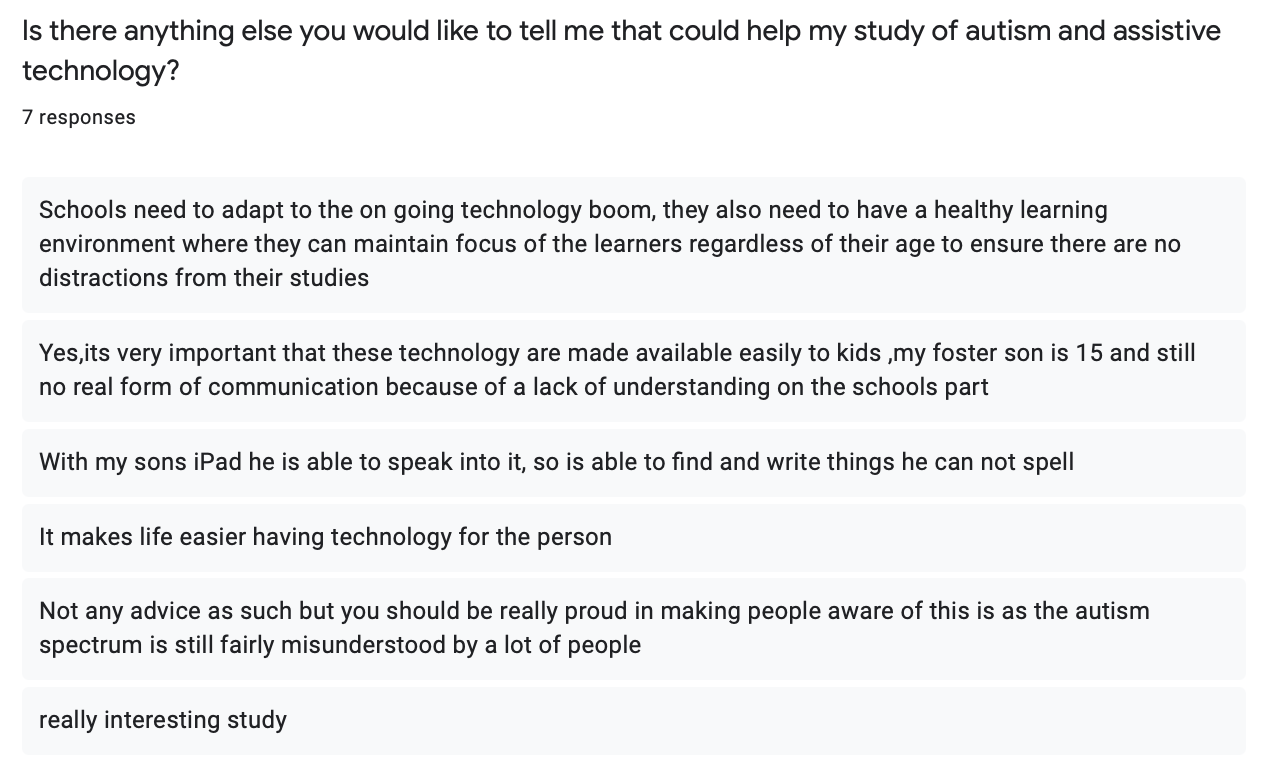
\includegraphics[width=1.0\textwidth]{IDD_LauraMartin_R00124705/Figures/furtherhelp.png}
\caption{Further information answer box}
{For question seventeen, 7 respondents gave their feedback of information that may further help my study.}
\end{figure}

\subsection{Survey two analysis}

\begin{table} [b]
    \centering
\begin{tabular}{ | m{3em} | m{10cm}| } 
\hline
Q1. & There is a good range of occupations that are related to the target audience. \\ 
\hline
Q.2 & This question gave the details of the participants, it concluded of their name and email address for further contact. \\ 
\hline
Q.3 & 100 percent of the participants educates a person with Autism, this is crucial for feedback and design going foreword.  \\ 
\hline
Q.4 & 83.3 percent of the respondents educated children with Autism who were the school going age of 4-11, this is vital information as that is the age of the demographic for the proposed application.  \\ 
\hline
Q.5 & 83.3 percent of the respondents educated children in a mixed gender school, while 16.7 percent taught in a all male school. This is interesting feedback as none of the applicants educated in an all female school.  \\ 
\hline
Q.6 & 83.3 percent of the respondents claimed their students struggled with either their homework or their school work and 16.7 percent had some difficulty. This result was to be expected as the Children are learning new skills and having a learning disability typically can make this challenging.   \\ 
\hline
Q.7 & 87.5 percent of the participants use technology in the class while 12.5 percent only sometimes use technology, this can be put down to limitations, resources and internet connection in the school. \\ 
\hline
Q.8 & All respondents explained what devices they used in the classroom, the most common answer was a form of tablet and an interactive whiteboard. \\ 
\hline
Q.9 & 100 percent of the respondents used a form of technology for educating students with Autism. \\ 
\hline
Q.10 & The respondents explained what form of devices they used to educate a student with Autism, the most common answer was an interactive whiteboard and a form of table. \\ 
\hline
Q.11 & 100 percent of the respondents used a child centered approach when educating students with Autism, this is expected as it is a recommend form of practice for individuals with Autism as ability can vary. \\ 
\hline
Q.12 & 75 percent of respondents used the internet as part of their studies, while 25 percent did not. This is interesting as due to the COVID-19 pandemic all schools in Ireland for a period of time had to migrate to teaching online. \\ 
\hline

Q.13 & Respondents gave an explanation as to why students would access the internet as part of their studies, the main reasons were accessing information for a project, or using the internet to access the curriculum or SeeSaw, an online learning portal for schools.  \\
\hline
Q.14 & 50 percent of respondents used a camera as part of their studies, while 50 percent did not. This was interesting as half the respondents did not use a camera to track students progress while education was online.  \\
\hline
Q.15 & 50 percent of respondents used a smart device camera as part of their studies, while 50 percent did not. This is not surprising as the same results appeared in question 14.  \\
\hline
\end{tabular}
\centering

\caption{Survey two analysis}
    \label{tab:my_label}
\end{table}




